\chapter{Tracce d'esame svolte - 2025}


\section{Esame del 15 gennaio 2025}

\subsection*{Esercizio 1}

Se $\varphi \to \psi$ è una tautologia e $\psi$ è una contraddizione, cosa possiamo concludere su $\varphi$?

\begin{center}
\begin{tabular}{c|c|c}
$\varphi$ & $\psi$ & $\varphi \to \psi$ \\
\hline
V & V & V \\
V & F & F \\
F & V & V \\
F & V & V
\end{tabular}
\end{center}

Se $\psi$ è una contraddizione, quindi sempre F, e $\varphi \to \psi$ una tautologia, allora $\psi$ sarà F.

\subsection*{Esercizio 3}

\subsubsection*{(i) Verificare che $(A, \oplus, *)$ è un anello}

Definiamo, in $A = \mathbb{Q} \times \mathbb{Q}$, le operazioni binarie $\oplus$ e $*$ ponendo, per ogni $a, b, x, y \in \mathbb{Q}$:
$$(a,b) \oplus (x,y) = (a+x, b+y); \qquad (a,b) * (x,y) = (0, ax).$$

\subsubsection*{Considerazioni sulla 1° operazione}

Visto che alla fine è un'addizione sarà sicuramente commutativo, associativo e avrà neutro sia a sx che a dx che sarà 0. Ogni elemento è invertibile perché siamo in Q, quindi è un gruppo abeliano

\subsubsection*{Considerazioni sulla 2° operazione}

\begin{align*}
\text{ASS: } [(a,b) * (x,y)] * (l,l) &\Leftrightarrow (a,b) * [(x,y) * (l,l)] \\
(0, ax) * (l,l) &\Leftrightarrow (a,b) * (0, xl) \\
(0, axl) &\Leftrightarrow (0, axl) \quad \text{è ASS}
\end{align*}

\subsubsection*{Considerazioni sulla distributività della 2° operazione rispetto alla 1°}

\begin{align*}
(a,b) * ((c,d) \oplus (x,l)) \\
((a,b) * (c,d)) \oplus ((a,b) * (x,l)) &\quad A \text{ SX va fatta la stessa cosa} \\
(0, ac) \oplus (0, ax) &\Leftrightarrow (0, az + ax) \\
(a,b) * ((c+x, d+l)) &\Leftrightarrow (0, ac + ax)
\end{align*}

\text{Sono uguali}

\subsubsection*{(ii) Decidere se $(A, \oplus, *)$ è unitario, se è commutativo, se è booleano, se è integro}

\textbf{Unitario:} Se $(A,*)$ è un monoide
$$(1,1) * (x,y) \Leftrightarrow (x,y) * (1,1)$$
$$(0,x) \Leftrightarrow (0,x)$$
Non è un monoide perché non ha neutro.

\textbf{È commutativo:} se $(A,\oplus)$ e $(A,*)$ lo sono, lo è:
$$(a,b) * (x,y) \Leftrightarrow (x,y) * (a,b)$$
$$(0,ax) \Leftrightarrow (0,xa) \quad \checkmark$$

\textbf{È booleano se:} è idempotente (ovvero $x^2 = x$) e unitario. Già abbiamo verificato che è unitario ma non idempotente

\textbf{Integro se} $(A,*)$ ha la LAP, quindi vale che:
$$\forall x, y \in S (x * y = 0_A \Rightarrow x = 0_A \lor y = 0_A)$$

Questo non è valido per tutte le coppie quindi non è integro. Infatti $(0,1) * (1,0) = (0,0)$ quindi non vale la LAP perché abbiamo ottenuto $(0,0)$ anche se le coppie $x*y$ non sono $0_A$.

\subsubsection*{(iii) Di ciascuno tra $(5,3)$ e $(5,0)$ stabilire se è un divisore dello zero in $(A, \oplus, *)$}

$(5,3)$ è divisore dello 0 in $(A, \oplus, *)$ se
$$\exists y \in A : x * y = 0_A \land x \neq 0_A \land y \neq 0_A$$

$$(5,3) * (x,y) = (0,5x) \quad \text{non mi dà } (0,0)$$

$$(5,0) * (x,y) = (0,0) \quad \text{ok } SX$$

$$(x,y) * (5,0) = (0,x) \quad \text{ok divisore dello 0 } DX$$

\subsubsection*{(iv) $B := \{0\} \times \mathbb{Z}$ è un sottoanello di $(A, \oplus, *)$? Nel caso, $B$ è isomorfo all'anello $(\mathbb{Z}, +, \cdot)$ degli interi? Rispondere alle stesse domande per $C := \mathbb{Z} \times \{0\}$ al posto di $B$}

È un sottoanello se presi $(0, \langle \text{elem } \mathbb{Z} \rangle)$ con la 1ª e 2ª operazione dell'anello mi dà sempre roba dell'anello $B$. In questo caso se uno ci pensa visto che la 1ª operazione è un'addizione la 1ª operazione darà sempre elementi di $B$, idem la 2ª. Ma se prendo $(0,1) * (0,1) = (0,0)$, $B$ non è integro come $\mathbb{Z}$ allora $B$ non è isomorfo a $\mathbb{Z}$. Perché ti ricordo che se l'insieme $B$ non ha le stesse proprietà dell'insieme originale $\mathbb{Z}$ allora $B$ non è isomorfo a $\mathbb{Z}$.

$B$ isomorfo all'anello $(\mathbb{Z}, +, \cdot)$? NO

Se rifaciamo lo stesso prova per $C$ vale lo stesso per $C$ NO perché presi 2 elementi $(1,0) * (3,0) = (0,3) \notin C$.

\subsection*{Esercizio 4}

Sia $a = \{n \in \mathbb{N} \mid n < 10\}$ e $f$ l'applicazione
$$x \in \mathcal{P}(a) \longmapsto \begin{cases}
|x| & \text{se } \exists x \notin a \\
1, & \text{se } 5 \in x
\end{cases} \quad x \in \mathbb{N}$$

\subsubsection*{(i) $f$ è iniettiva? $f$ è suriettiva?}

Una funzione è iniettiva se per 1 elemento del dominio c'è solo 1 elemento del codominio. Esplicitiamo l'insieme $a$:
$$a = \{0, 1, 2, 3, 4, 5, 6, 7, 8, 9\}$$

Se scelgo $\{0,5\}$ e $\{1,5\}$ diversi elementi del dominio puntano allo stesso elemento del codominio quindi non è sicuramente iniettiva.

Una funzione è suriettiva se per TUTTI gli elementi del codominio c'è ALMENO 1 elemento del dominio. L'immagine di $f$ non è uguale ad $\mathbb{N}$ infatti, per questa funzione elementi come 11, 12, 13 non verranno mai raggiunti quindi non è suriettiva.

\subsubsection*{(ii) Determinare l'immagine im $f = f(\mathcal{P}(a))$ di $f$}

$\mathcal{P}(a)$ sappiamo tutte le combinazioni possibili di $a$, in:

$\{0,5\}, \{2,5\}, \{2,5\} \dots \{0,1,5\}, \{0,2,5\}, \dots$ quindi

$$\text{im } f = f(\mathcal{P}(a)) = \{0, 1, 2, 3, 4, 5, 6, 7, 8, 9\}$$

Dato $\rho$ il nucleo di equivalenza di $f$.

\textbf{(iii)} Determinare le classi $[\{1,2\}]_\rho$ e $[5]_\rho$, indicandone il numero di elementi:

$$\{\{1,2\}\}_\rho = \{y \in a : f(\{1,2\}) = f(y)\} = 2 \quad \text{tutte le combinaz di 2 elementi tranne 5}$$

Quindi $\mathcal{P}(a) = \binom{9}{2} = \frac{9!}{2! \cdot 7!} = \frac{9 \cdot 8}{2} = 9 \cdot 4 = 36$

$$\{\{5\}\}_\rho = \{y \in a : f(\{5\}) = f(y)\} = 2^9 + 9$$

quindi se volessi un po' semplificare il ragionamento direi: $2^9$ perché considero 5 come elemento fisso + 9 (singletone di tutti gli altri elementi da 0-9 tranne 5)

\subsubsection*{(iv) Calcolare $|\mathcal{P}(a)/\rho|$}

Usando il teorema dell'omomorfismo tra insiemi la cardinalità di Im $f$ che è $\{0, 1, 2, 3, 4, 5, 6, 7, 8, 9\}$ allora la cardinalità di $|\mathcal{P}(a)/\rho|$ è 10. Perché il vuoto non lo conti separato? Perché se $x = \emptyset$ allora $|x| = 0$ quindi fa parte della funzione.

\subsection*{Esercizio 5}

Per ogni $p \in P := \{2,3,5\}$ e $n \in \mathbb{N}^* = \mathbb{N} \setminus \{0\}$, indichiamo con $f_p(n)$ l'esponente della massima potenza di $p$ che divide $n$, e sia $f(n) = \sum_{p \in P} f_p(n)$. Siano $\sigma$ e $\rho$ le relazioni binarie in $\mathbb{N}^*$ definite da: per ogni $a, b \in \mathbb{N}^*$:
$$a \,\sigma\, b \leftrightarrow (a = b \lor \forall p \in P\, (p|a \to p^2|b))$$
e
$$a \,\rho\, b \leftrightarrow (\forall p \in P\, (p^{f_p(a)}|b) \land (a = b \lor f(a) < f(b))).$$

\subsubsection*{(i) Di ciascuna di $\sigma$ e $\rho$ stabilire se è una relazione d'ordine}

Per entrambe le relazioni non è verificata la relazione d'ordine:

\begin{itemize}
    \item Per $\sigma$: se proviamo la simmetria per 4 e 8 non è verificata.
    
    \item Per $\rho$: se proviamo la simmetria per 2 e 14 non è verificata.
\end{itemize}

\section {Esame del 20 febbraio 2025}

\subsection*{Esercizio 1}

\subsubsection*{(i) Dare la definizione di numero primo in $\mathbb{Z}$}

Tutti i numeri divisibili solo per 1 e per sé stesso tranne: $-1, 0$ e $1$.

\subsubsection*{(ii) Posto $S = \{-2, -1, 0, 1, 2, 3, 4\}$, determinare il numero dei sottoinsiemi di $S$ che contengono tutti i numeri primi appartenenti ad $S$}

$$\{-2, 2, 3\} \quad 2^3 = 8$$

Eliminando i numeri non considerati primi: $-1, 0$ e $1$ allora $2^3$ saranno tutte le combinazioni possibili.

\subsubsection*{(iii) Quanti sono i sottoinsiemi di $S$ che hanno ordine 3?}

$$\mathcal{P}_3(S) = \binom{m}{k} = \frac{n!}{k!(n-k)!} = \binom{7}{3} = \frac{7!}{3! \cdot 4!} = \frac{7 \cdot 6 \cdot 5}{3} = 7 \cdot 3 \cdot 5 = 105$$

\subsection*{Esercizio 4}

\subsubsection*{(i) Perché $f$ è ben definita?}

Per il teorema dell'aritmetica che assicura ciò è ben definito da 2 in poi per $n = 1$ qualunque sequenza di primi deve essere 0 e quindi ben definito.

\subsubsection*{(ii) $f$ è iniettiva? È suriettiva?}

In questo caso, $f(2) = f(3)$ quindi NON iniettiva.

Suriettiva quando ogni elemento del codominio ha ALMENO 1 corrispondenza nel dominio. È SURIETTIVA perché per ogni $n$, $f(3^n) = n$.

\subsubsection*{(iii) Determinare $\tilde{f}(\{0\})$, $\tilde{f}(\{1\})$, $\tilde{f}(\{8h \mid h \in \mathbb{N}^*\})$}

$$\tilde{f}(\{8h \mid h \in \mathbb{N}^*\}) = \{3, 4, 5, \ldots\} = \{n \in \mathbb{N} \mid n \geq 3\}$$

\subsubsection*{(iv) Verificare che $f$ determina un omomorfismo da $(\mathbb{N}^*, \cdot)$ a $(\mathbb{N}, +)$}

\begin{align*}
n_1 &= p_1^{\alpha_1} \cdots p_t^{\alpha_t} \\
n_2 &= p_1^{\beta_1} \cdots p_t^{\beta_t} \\
f(n_1 \cdot n_2) &= f(p_1^{\alpha_1 + \beta_1} \cdots p_t^{\alpha_t + \beta_t}) \\
&= \sum_{i=1}^{t} (\alpha_i + \beta_i) = \sum_{i=1}^{t} \alpha_i + \sum_{i=1}^{t} \beta_i = f(n_1) + f(n_2)
\end{align*}

\text{Sì è un omomorfismo}

\subsubsection*{(v) Indicato con $\Re$ il nucleo di equivalenza di $f$ (cioè l'equivalenza associata a $f$), determinare $[8]_\Re$}

$$[8]_{\Re} = \{y \in \mathbb{N}^* \mid 8 \Re y\} = \{y \in \mathbb{N}^* \mid f(8) = f(y)\}$$

Il numero $y$ la cui $f(y) = 3$ potrebbe essere un qualsiasi numero $y$ tranne 0 la cui somma della scomposizione in numeri primi mi dia 3. Quindi:
Siano $p_1, p_2, p_3$ numeri interi positivi e $a_1, a_2, a_3 \in \mathbb{N}$

$$= \{n \in \mathbb{N} \mid n = p_1 p_2 p_3\}$$

\subsubsection*{(vi) Determinare in $(\mathbb{N}^*, \sigma)$ eventuali minimo, massimo, elementi minimali, elementi massimali}

Sia $\sigma$ la relazione d'ordine definita in $\mathbb{N}^*$ da: per ogni $a, b \in \mathbb{N}^*$
$$a \,\sigma\, b \Longleftrightarrow (a = b \lor f(a) \text{ è un divisore proprio di } f(b)).$$

Sicuramente non ci saranno elementi massimali, massimi e minimi. Mentre i minoranti saranno tutti gli $n$ con $f(n) = 1$ (numeri primi).

\subsubsection*{(vii) Determinare in $(\mathbb{N}^*, \sigma)$ l'insieme dei minoranti di $\{4, 9\}$}

%\begin{center}
%\begin{tikzpicture}

%\end{tikzpicture}

%\end{center}

$$MINOR(\{4, 9\})_{(\mathbb{N}^*, \sigma)} = \mathbb{P} \{\text{primi pos}\}$$

\subsubsection*{(viii) Dopo aver dato la definizione di reticolo, si dica se $(\mathbb{N}^*, \sigma)$ è un reticolo}

$$\forall x, y \in \mathbb{N}^* \left( \exists \sup(\{x, y\}) \land \exists \inf(\{x, y\}) \right)$$

NON è un reticolo, prendi come esempio il SUP tra 8 e 4, non esiste.

\subsubsection*{(ix) Posto $L = \{1, 2, 6, 9, 12, 25, 30\}$, scegliere un $a \in L$ in maniera tale che $(L \setminus \{a\}, \sigma)$ risulti essere un reticolo}

\begin{center}
	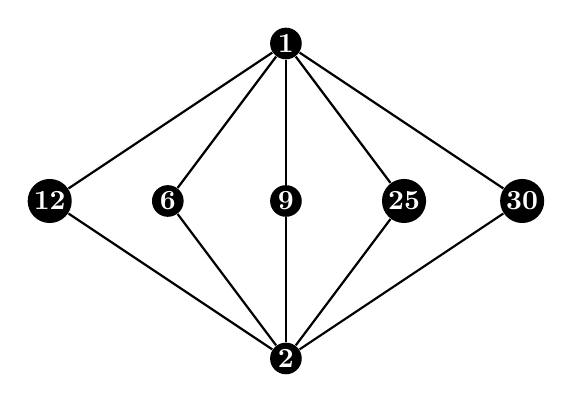
\begin{tikzpicture}[
		% Stile globale per i nodi, li rende piccoli pallini pieni neri
		% Se vuoi solo il testo, rimuovi 'fill' e 'inner sep' e usa 'draw' per un contorno:
		% node style/.style={circle, draw=black, minimum size=6mm, inner sep=0pt, font=\bfseries}
		node style/.style={circle, fill=black, inner sep=1pt, minimum size=3pt, font=\bfseries\color{white}},
		% Stile per le linee (archi)
		edge style/.style={thick, color=black}
	]

	% =================================
	% LIVELLO 1 (In alto)
	% =================================
	\node[node style] (n1) at (0, 3) {1};

	% =================================
	% LIVELLO 2 (Intermedio)
	% =================================
	% Posizionamento dei nodi del secondo livello
	% Le coordinate sono state scelte per replicare l'allineamento orizzontale
	\node[node style] (n12) at (-3, 1) {12};
	\node[node style] (n6) at (-1.5, 1) {6};
	\node[node style] (n9) at (0, 1) {9};
	\node[node style] (n25) at (1.5, 1) {25};
	\node[node style] (n30) at (3, 1) {30};

	% =================================
	% LIVELLO 3 (In basso)
	% =================================
	\node[node style] (n2) at (0, -1) {2};

	% =================================
	% CONNESIONI (Archi)
	% =================================

	% Connessioni dal LIVELLO 1 al LIVELLO 2
	\draw[edge style] (n1) -- (n12);
	\draw[edge style] (n1) -- (n6);
	\draw[edge style] (n1) -- (n9);
	\draw[edge style] (n1) -- (n25);
	\draw[edge style] (n1) -- (n30);

	% Connessioni dal LIVELLO 2 al LIVELLO 3
	\draw[edge style] (n12) -- (n2);
	\draw[edge style] (n6) -- (n2);
	\draw[edge style] (n9) -- (n2);
	\draw[edge style] (n25) -- (n2);
	\draw[edge style] (n30) -- (n2);
	
	\end{tikzpicture}
\end{center}

\text{a potrebbe essere qualsiasi numero tranne 1 e 2}

\subsection*{Esercizio 5}

Definiamo l'operazione binaria $*$ in $\mathcal{P}(\mathbb{N})$ ponendo $\forall x, y \in \mathcal{P}(\mathbb{N})(x * y = x \cup (y \setminus \{3\}))$.

\subsubsection*{(i) Decidere se $*$ è commutativa e se è associativa}

$$x * y = y * x \Leftrightarrow x \cup (y \setminus \{3\}) = y \cup (x \setminus \{3\}) \quad \text{No comm}$$

$$x = \{1, 2, 3\} \quad y = \{4, 5\} \qquad \{1, 2, 3, 4, 5\} = \{1, 2, 4\}$$

\textbf{ASS:} $(x * y) * z = x * (y * z)$

$$(x \cup (y \setminus \{3\})) * z = x * (y \cup (z \setminus \{3\}))$$

$$(x \cup (y \setminus \{3\})) \cup (z \setminus \{3\}) = x \cup ((y \cup (z \setminus \{3\})) \setminus \{3\})$$

Per le proprietà dell'unione possiamo rimuovere le parentesi

$$x \cup (y \setminus \{3\}) \cup (z \setminus \{3\}) = x \cup (y \cup (z \setminus \{3\})) \setminus \{3\}$$

hanno lo stesso significato quindi è associativa.

\subsubsection*{(ii) Determinare gli eventuali elementi neutri a destra, a sinistra, neutri in $(\mathcal{P}(\mathbb{N}), *)$}

$$\exists x : \emptyset * y = y \setminus \{3\} \longrightarrow \text{Non ha neutro}$$

$$\exists x : y * \{3\} = y$$

\subsubsection*{(iii) Stabilire se $(\mathcal{P}(\mathbb{N}), *)$ è un semigruppo, un monoide, un gruppo}

semigruppo commutativo

\subsubsection*{(iv) Determinare gli elementi cancellabili a sinistra o a destra e gli elementi idempotenti in $(\mathcal{P}(\mathbb{N}), *)$}

\textbf{Cancellabile SX:} $a * x = a * y \to x = y$

$$a \cup (x \setminus \{3\}) = a \cup (y \setminus \{3\}) \to x = y$$

Quando $a = \emptyset$

\textbf{Cancellabile a DX:} $x * a = y * a \to x = y$, quando $a = \{3\}$

\textbf{Idempotente:} $\{3\} * \{3\} = \{3\} \cup \emptyset = \{3\}$

\subsubsection*{(v) L'operazione $\cap$ in $\mathcal{P}(\mathbb{N})$ è distributiva a sinistra rispetto a $*$? E a destra?}

\textbf{SX:} $a \cap (b * c) \Leftrightarrow (a \cap b) * (a \cap c)$

$$a \cap (b \cup (c \setminus \{3\})) \Leftrightarrow (a \cap b) \cup ((a \cap c) \setminus \{3\})$$

$$(a \cap b) \cup (a \cap c \setminus \{3\}) \Leftrightarrow (a \cap b) \cup (a \cap c \setminus \{3\}) \qquad ok?$$

\textbf{DX:} $(b * c) \cap a \Leftrightarrow (b \cap a) * (c \cap a)$

$$(b \cup (c \setminus \{3\})) \cap a \Leftrightarrow (b \cap a) \cup (c \cap a) \setminus \{3\}$$

$$a \cap b \cup a \cap c \setminus \{3\} \Leftrightarrow b \cap a \cup c \cap a \setminus \{3\} \qquad ok?$$

sì sono distributivi

\subsection*{Esercizio 6}

Determinare l'insieme dei numeri interi $n$ tali che $84n + 5 \equiv_{92} 14n - 1$.

$$84n + 14n \equiv 92 - 1 - 5$$
$$70n \equiv 92 - 6 \longrightarrow 70n \equiv 43 \qquad MCD(70, 92) = 2 \mid 86$$
\text{Perché 2 divide 86 ci saranno soluzioni}
$$35n \equiv_{46} 43 \longrightarrow 35n \equiv_{46} 1$$
$$46 = 35 \cdot 1 + 11 \qquad 11 = 46 + 35 \cdot 1$$
$$35 = 11 \cdot 3 + 2 \qquad 2 = 35 - 11 \cdot 3$$
$$11 = 2 \cdot 5 + 1 \qquad 1 = 11 - 2 \cdot 5$$
$$1 = 11 - 5(35 - 11 \cdot 3) = 11 \quad -5 \cdot 35 \qquad +11 \cdot 3 \cdot 5$$
$$11(1 + 15) + 35(-5) \longrightarrow 16(46 - 35) + 35(-5)$$
$$\longrightarrow 46 \cdot 16 + 35(-16) + 35(-5) \longrightarrow 35(-21) + 46 \cdot 16$$
$$35(25) + 46 \cdot 16$$
\text{Abbiamo portato il -21 in modulo 46 aggiungendo +46}
$$\{35\}_{46} \{25\}_{46} n = \{43\}_{46}, \{25\}_{46}$$
$$n = \{17\}_{46}$$

\section{Esame del 14 marzo 2025}

\subsection*{Esercizio 1. Sia $\star$ l'operazione binaria definita in $\mathbb{Z}_{21}$ ponendo, per ogni $a, b \in \mathbb{Z}_{21}$,
$$ \overline{a} \star \overline{b} = \overline{3ab} + \overline{10}(\overline{a} - \overline{b}) + \overline{2}. $$}

\subsubsection*{(i) $\star$ è associativa? È commutativa?}

\textbf{Commutatività:}
L'operazione $\star$ è commutativa se e solo se $\overline{a} \star \overline{b} = \overline{b} \star \overline{a}$ per ogni $\overline{a}, \overline{b} \in \mathbb{Z}_{21}$.
\begin{align*}
\overline{a} \star \overline{b} &= \overline{3ab} + \overline{10a} - \overline{10b} + \overline{2} \\
\overline{b} \star \overline{a} &= \overline{3ba} + \overline{10b} - \overline{10a} + \overline{2}
\end{align*}
Affinché $\overline{a} \star \overline{b} = \overline{b} \star \overline{a}$, dobbiamo avere:
$$ \overline{10a} - \overline{10b} \equiv \overline{10b} - \overline{10a} \pmod{21} $$
$$ \overline{20a} \equiv \overline{20b} \pmod{21} $$
Poiché $\overline{20} \equiv \overline{-1} \pmod{21}$:
$$ \overline{-a} \equiv \overline{-b} \pmod{21} \implies \overline{a} \equiv \overline{b} \pmod{21} $$
L'operazione $\star$ è commutativa \textbf{solo se} $\overline{a} = \overline{b}$. Poiché non vale per ogni coppia, l'operazione $\star$ \textbf{non è commutativa}.

\textbf{Associatività:}
Controesempio: $\overline{1}, \overline{0}, \overline{0}$.
$$ (\overline{1} \star \overline{0}) \star \overline{0} = \overline{12} \star \overline{0} = \overline{3(12)(0)} + \overline{10}(\overline{12} - \overline{0}) + \overline{2} = \overline{122} \equiv \overline{17} \pmod{21} $$
$$ \overline{1} \star (\overline{0} \star \overline{0}) = \overline{1} \star \overline{2} = \overline{3(1)(2)} + \overline{10}(\overline{1} - \overline{2}) + \overline{2} = \overline{6} - \overline{10} + \overline{2} = \overline{-2} \equiv \overline{19} \pmod{21} $$
Poiché $\overline{17} \ne \overline{19}$, l'operazione $\star$ \textbf{non è associativa}.

\vspace{0.3cm}
\hrule
\vspace{0.3cm}

\subsubsection*{(ii) Determinare l'eventuale elemento neutro di $(\mathbb{Z}_{21}, \star)$.}

Si cerca un elemento neutro $\overline{e}$ tale che $\overline{a} \star \overline{e} = \overline{a}$ e $\overline{e} \star \overline{a} = \overline{a}$.

\textbf{Ricerca del Neutro Destro ($\overline{a} \star \overline{e} = \overline{a}$):}
$$ e(3a - 10) \equiv -9a - 2 \pmod{21} $$
Se $\overline{a}=\overline{0}$, si trova $\overline{-10e} \equiv \overline{-2} \implies \overline{11e} \equiv \overline{19} \implies \overline{e} = \overline{17}$.
Verifica con $\overline{a}=\overline{1}$:
$$ \overline{17}(\overline{3} - \overline{10}) \equiv \overline{17} \cdot \overline{-7} = \overline{-119} \equiv \overline{7} \pmod{21} $$
Mentre $\overline{-9a} - \overline{2} = \overline{-9} - \overline{2} = \overline{-11} \equiv \overline{10} \pmod{21}$. Poiché $\overline{7} \ne \overline{10}$, la condizione fallisce.

\textbf{Ricerca del Neutro Sinistro ($\overline{e} \star \overline{a} = \overline{a}$):}
$$ e(3a + 10) \equiv 11a - 2 \pmod{21} $$
Se $\overline{a}=\overline{1}$, si trova $\overline{13e} \equiv \overline{9} \implies \overline{e} = \overline{18}$.
Verifica con $\overline{a}=\overline{0}$:
$$ \overline{18}(\overline{10}) = \overline{180} \equiv \overline{12} \pmod{21} $$
Mentre $\overline{11a} - \overline{2} = \overline{-2} \equiv \overline{19} \pmod{21}$. Poiché $\overline{12} \ne \overline{19}$, la condizione fallisce.

\textbf{Conclusione:} L'elemento neutro \textbf{non esiste}.
Di conseguenza: a.) \textbf{nessun} elemento è invertibile; b.) $(\mathbb{Z}_{21}, \star)$ \textbf{non è un gruppo}.

\vspace{0.3cm}
\hrule
\vspace{0.3cm}

\subsubsection*{(iii) $\{\overline{0}\}$ è una parte chiusa in $(\mathbb{Z}_{21}, \star)$?}

Verifichiamo se $\overline{0} \star \overline{0} \in \{\overline{0}\}$:
$$ \overline{0} \star \overline{0} = \overline{3(0)(0)} + \overline{10}(\overline{0} - \overline{0}) + \overline{2} = \overline{2} $$
Poiché $\overline{2} \ne \overline{0}$, l'insieme $\{\overline{0}\}$ \textbf{non è una parte chiusa} in $(\mathbb{Z}_{21}, \star)$.

\vspace{0.5cm}
\hrule
\vspace{0.5cm}

\subsection*{Esercizio 2}

Sia $A = \{n \in \mathbb{N} \mid n < 10\}$ e sia $E$ l'insieme delle relazioni di equivalenza $\sigma$ in $A$ tali che $1 \sigma 7$ e $\overline{1}_{\sigma} \cap \overline{3}_{\sigma} \neq \emptyset$. Vero o falso (e perché)?
Dalle condizioni $1 \sigma 7$ e $\overline{1}_{\sigma} \cap \overline{3}_{\sigma} \neq \emptyset$, si deduce che per ogni $\sigma \in E$:
$$ \overline{1}_{\sigma} = \overline{7}_{\sigma} = \overline{3}_{\sigma} $$
Gli elementi $\{1, 3, 7\}$ devono stare nella stessa classe di equivalenza. Usiamo il teorema delle relazioni d'equivalenza per svolgere l'esercizio

\subsubsection*{(i) Per ogni $X \subseteq A$ tale che $\{1, 2, 3, 7, 8\} \subseteq X$ esiste $\sigma \in E$ tale che $X = \overline{3}_{\sigma}$.}

Consideriamo il sottoinsieme minimo specificato: $X_0 = \{1, 2, 3, 7, 8\}$. Vogliamo dimostrare che esiste una relazione $\sigma \in E$ tale che $X_0$ sia la classe $\overline{3}_{\sigma}$.

1.  \textbf{Partizione $\mathcal{P}$:} Possiamo costruire una partizione $\mathcal{P}$ di $A$ tale che $X_0$ sia un blocco (una classe di equivalenza). L'insieme degli elementi rimanenti è $A \setminus X_0 = \{4, 5, 6, 9\}$.
    $$\mathcal{P} = \{ X_0, \{4\}, \{5\}, \{6\}, \{9\} \}$$
2.  \textbf{Verifica della Condizione $E$:} La partizione $\mathcal{P}$ definisce una relazione $\sigma$.
    \begin{itemize}
        \item Poiché $\{1, 3, 7\} \subset X_0$, tutte le classi $\overline{1}_{\sigma}, \overline{3}_{\sigma}, \overline{7}_{\sigma}$ sono uguali a $X_0$.
        \item Dunque, $1 \sigma 7$ è soddisfatta.
        \item Dunque, $\overline{1}_{\sigma} \cap \overline{3}_{\sigma} = X_0 \cap X_0 = X_0 \neq \emptyset$ è soddisfatta.
    \end{itemize}
    Pertanto, $\sigma \in E$.
3.  \textbf{Verifica della Condizione $X = \overline{3}_{\sigma}$:} Per costruzione, $\overline{3}_{\sigma} = X_0$.

Dunque, \textbf{esiste} $\sigma \in E$ tale che $X_0 = \overline{3}_{\sigma}$.

\vspace{0.3cm}
\hrule
\vspace{0.3cm}

\subsubsection*{(ii) Per ogni $X \subseteq A$ tale che $\{1, 2, 3, 7, 8\} \subseteq X$ esiste $\sigma \in E$ tale che $X = \overline{2}_{\sigma}$.}
\textbf{VERO}.
Sia $X = \{1, 2, 3, 7, 8\}$. Vogliamo $\overline{2}_{\sigma} = X$.
Poiché $1 \in X$ e $2 \in X$, la classe $\overline{2}_{\sigma}$ deve contenere $\overline{1}_{\sigma}$.
In una partizione $\mathcal{P} = \{X, \{4\}, \{5\}, \{6\}, \{9\}\}$, si ha $\overline{2}_{\sigma} = X$.
Inoltre, $\overline{1}_{\sigma} = \overline{3}_{\sigma} = \overline{7}_{\sigma} = X$, quindi $\sigma \in E$ è soddisfatta.

\vspace{0.3cm}
\hrule
\vspace{0.3cm}

\subsubsection*{(iii) Per ogni $X \subseteq A$ tale che $\{1, 2, 3\} \subseteq X$ esiste $\sigma \in E$ tale che $X = \overline{2}_{\sigma}$.}
\textbf{FALSO}.
Se $X$ è la classe $\overline{2}_{\sigma}$, e $\overline{1}_{\sigma} \subseteq X$, allora deve valere $\overline{1}_{\sigma} = \overline{7}_{\sigma} = X$.
Se $X = \{1, 2, 3\}$, allora $\overline{7}_{\sigma} = \{1, 2, 3\}$, il che è assurdo poiché $7 \notin \{1, 2, 3\}$. Non esiste $\sigma \in E$ con $X = \overline{2}_{\sigma}$ in questo caso.

\vspace{0.3cm}
\hrule
\vspace{0.3cm}

\subsubsection*{(iv) Esiste $\sigma \in E$ tale che $\overline{2}_{\sigma} = \{2, 9\}$;}
\textbf{VERO}.
Dobbiamo costruire una partizione $\mathcal{P}$ in cui $\{2, 9\}$ sia una classe e $\{1, 3, 7\}$ stiano in un'altra classe.
Sia $B = \{1, 3, 7\}$. Il resto degli elementi è $R = A \setminus (B \cup \{2, 9\}) = \{4, 5, 6, 8\}$.
Una partizione è:
$$ \mathcal{P} = \{\{1, 3, 7\}, \{2, 9\}, \{4\}, \{5\}, \{6\}, \{8\}\} $$
In $\mathcal{P}$, $\overline{2}_{\sigma} = \{2, 9\}$ (OK) e $\overline{1}_{\sigma} = \overline{3}_{\sigma} = \overline{7}_{\sigma} = \{1, 3, 7\}$, quindi $\sigma \in E$ è soddisfatta.

\vspace{0.3cm}
\hrule
\vspace{0.3cm}

\subsubsection*{(v) $|E| = \binom{10}{3}$.}
\textbf{FALSO}.
Il numero di relazioni $|E|$ è il numero di partizioni dell'insieme $A' = \{\{1, 3, 7\}, 2, 4, 5, 6, 8, 9\}$, che ha 7 elementi. Se calcoliamo $\binom{10}{3} = 120$ 
potremmo capire intuitivamente che non è possibile che sia equivalente alla cardinalità delle partizioni infatti, 10 su 3 calcolerebbe in quanti modi possiamo inserire i 
10 elementi in 3 partizioni ma la nostra condizione è che 1, 3, 7 rimangano insieme, cosa che 10 su 3 non considera e quindi è FALSO.

\vspace{0.3cm}
\hrule
\vspace{0.3cm}

\subsubsection*{(vi) $|E| = 2^7$.}
\textbf{FALSO}.
Questa è un'altra affermazione falsa perché calcola in quanti modi possiamo disporre 7 elementi ma non considera che questi 7 elementi potrebbero stare nella
partizione indivisibile di 1, 3 e 7. Quindi FALSO

\vspace{0.5cm}
\hrule
\vspace{0.5cm}

\subsection*{Esercizio 4. Sia $S = \{a, \{a\}, b\}$, dove assumiamo $a \neq b \neq \{a\}$. Siano $T = \mathcal{P}(S) \times \mathcal{P}(S)$ e $f$ l'applicazione $f((x, y)) = |x \triangle y|$ con codominio $\{0, 1, 2, 3, 4, 5, 6\}$.}

\subsubsection*{(i) $f$ è iniettiva? È suriettiva?}

\textbf{Iniettività:}
Non è iniettiva. 
$$ f((\{a\}, \{\{a\}\})) = |\{a, \{a\}\}| = 2 $$
$$ f((\{a\}, \{b\})) = |\{a, b\}| = 2 $$
Poiché $(\{a\}, \{\{a\}\}) \ne (\{a\}, \{b\})$ ma $f$ ha lo stesso valore, \textbf{NON è INIETTIVA}.

\textbf{Suriettività:}
Poiché $|x \triangle y| \le |S| = 3$, l'immagine di $f$ è $\text{Im}(f) = \{0, 1, 2, 3\}$.
Il codominio è $\{0, 1, 2, 3, 4, 5, 6\}$. Gli elementi $\{4, 5, 6\}$ non sono mai raggiunti.
\textbf{NON è SURIETTIVA}.

\vspace{0.3cm}
\hrule
\vspace{0.3cm}

\subsubsection*{(ii) Determinare $f^{\leftarrow}(\{0\})$, $f^{\leftarrow}(\{3\})$, $f^{\rightarrow}(T)$.}

\paragraph*{Immagine inversa di $\{0\}$:}
$$ f^{\leftarrow}(\{0\}) = \{(x, y) \in T \mid |x \triangle y| = 0\} = \{(x, S \ x) \mid x \in \mathcal{P}(S)\} $$

\paragraph*{Immagine inversa di $\{3\}$:}
$$ f^{\leftarrow}(\{3\}) = \{(x, y) \in T \mid |x \triangle y| = 3\} $$
Poiché $|S|=3$, $|x \triangle y| = 3$ se e solo se $x$ e $y$ formano una partizione di $S$ (cioè $x \cap y = \emptyset$ e $x \cup y = S$).
$$ f^{\leftarrow}(\{3\}) = \{(x, S \setminus x) \mid x \in \mathcal{P}(S)\} $$

\paragraph*{Immagine diretta di $T$:}
$$ f^{\rightarrow}(T) = \{|x \triangle y| \mid x, y \in \mathcal{P}(S)\} = \{0, 1, 2, 3\} $$

\vspace{0.3cm}
\hrule
\vspace{0.3cm}

\subsubsection*{(iii) Determinare eventuali minimo, massimo, elementi minimali e massimali in $(T, \rho)$.}

La relazione d'ordine $\rho$ è definita da: $(x, y) \rho (z, t) \iff ((x, y) = (z, t) \lor f((x, y)) < f((z, t)))$.

\paragraph*{Elementi Minimali}
Sono le coppie con il valore minimo di $f$, ovvero $f((x, y)) = 0$.
$$ \text{Minimali} = \{(x, x) \mid x \in \mathcal{P}(S)\} $$
Ci sono $2^3 = \mathbf{8}$ elementi minimali (incomparabili tra loro). Non esiste un unico elemento minimo.

\paragraph*{Elementi Massimali}
Sono le coppie con il valore massimo di $f$, ovvero $f((x, y)) = 3$.
$$ \text{Massimali} = \{(x, S \setminus x) \mid x \in \mathcal{P}(S)\} $$
Ci sono $\mathbf{8}$ elementi massimali (incomparabili tra loro). Non esiste un unico elemento massimo.

\paragraph*{Minimo e Massimo}
\textbf{Minimo:} Non esiste. \textbf{Massimo:} Non esiste.

\vspace{0.3cm}
\hrule
\vspace{0.3cm}

\subsubsection*{(iv) Determinare in $(T, \rho)$ un sottoinsieme totalmente ordinato del massimo ordine possibile.}

Guardare lo svolgimento del 5° punto.

\vspace{0.3cm}
\hrule
\vspace{0.3cm}

\subsubsection*{(v) Disegnare un diagramma di Hasse di $L = \{(\{a\}, \{a\}), (\{a, b\}, \{a, b\}), (\{a\}, \{\{a\}\}), (\{a, b\}, \{\{a\}\})\}$ ordinato dalla relazione indotta da $\rho$.}

Gli elementi originali con i loro valori di $f$ sono:
$a = (\{a\}, \{a\})$
$b = (\{a, b\}, \{a, b\})$
$c = (\{a\}, \{\{a\}\})$
$d = (\{a, b\}, \{\{a\}\})$

\begin{figure}[h]
    \centering
    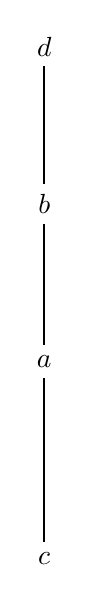
\begin{tikzpicture}[node distance=1.5cm, auto, thick, scale=1.0]
        % Nodi disposti verticalmente per formare una colonna
        \node (d_node) at (0, 7.0) {$d$};
        % \node (f3_label) at (0, 3.8) {}; % Spazio per livello 3 (non etichettato con f=3 nell'immagine)
        
		\node (b_node) at (0, 5.0) {$b$};

        \node (a_node) at (0, 3.0) {$a$};
		
		\node (c_node) at (0, 0.5) {$c$};
        % \node (f2_label) at (0, 1.8) {}; % Spazio per livello 2
		
        \draw (c_node) -- (a_node);
        \draw (a_node) -- (b_node);
		\draw (b_node) -- (d_node);
    \end{tikzpicture}
\end{figure}

\vspace{0.5cm}
\hrule
\vspace{0.5cm}

\subsection*{Esercizio 5. Decidere se $(p \to p) \to (((q \to (r \wedge s)) \leftrightarrow ((q \to r) \wedge (q \to s))))$ è una tautologia.}

\subsubsection*{Svolgimento}

La proposizione da analizzare è:
$$ (p \to p) \to (((q \to (r \wedge s)) \leftrightarrow ((q \to r) \wedge (q \to s)))) $$

La sotto-proposizione $p \to p$ è una tautologia ($\text{V}$). La proposizione si semplifica a:
$$ \text{V} \to (((q \to (r \wedge s)) \leftrightarrow ((q \to r) \wedge (q \to s)))) $$
Che è logicamente equivalente a:
$$ (q \to (r \wedge s)) \leftrightarrow ((q \to r) \wedge (q \to s)) $$

Questa è la nota \textbf{Proprietà Distributiva dell'Implicazione sulla Congiunzione}, che è un'equivalenza logica. Pertanto, la bicondizionale tra i due lati è sempre Vera.

\textbf{Conclusione:} La proposizione è una \textbf{tautologia}.
(La tabella di verità fornita è una verifica formale di questa equivalenza logica).

\section{Esame del 19 giugno 2025}
\begin{center}
    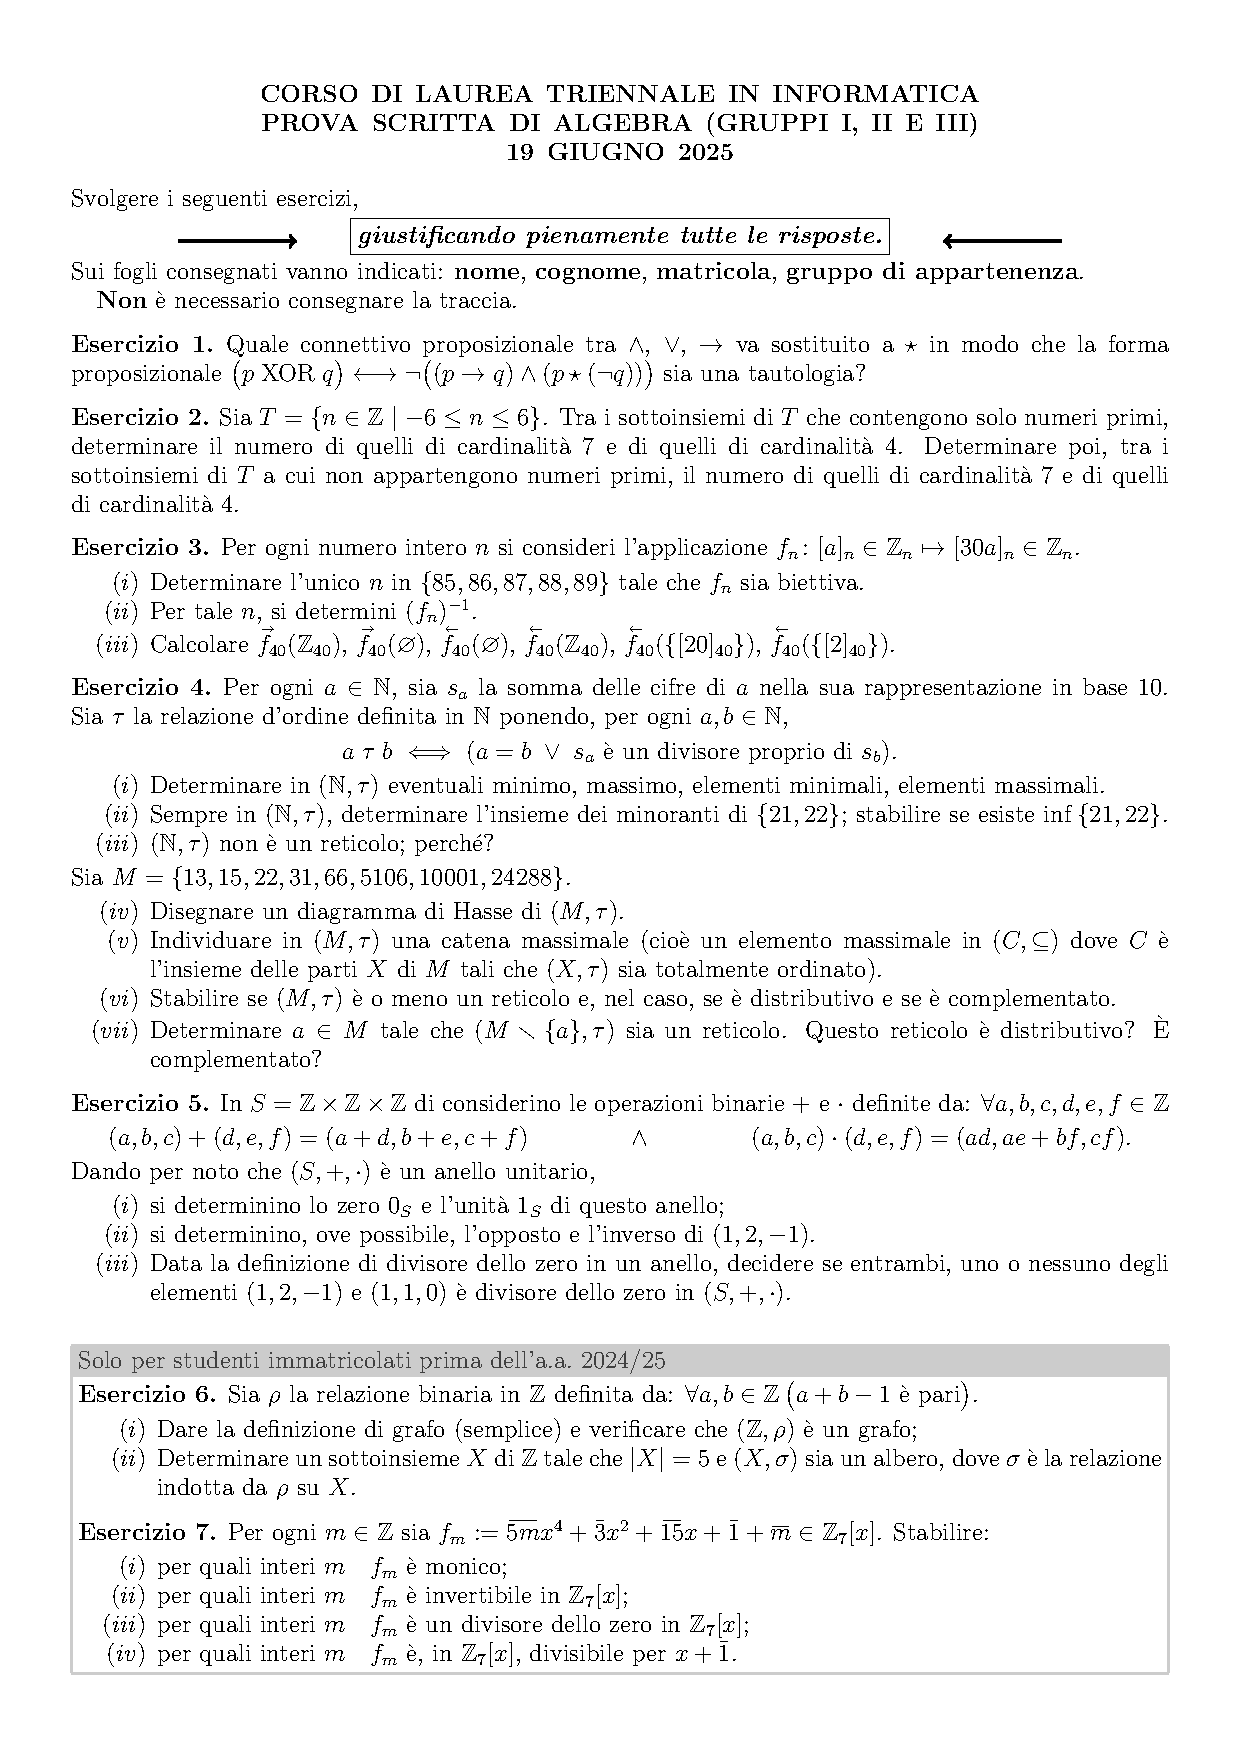
\includegraphics[scale=.85]{pdf/25-06-19.pdf}
\end{center}

\subsection*{Esercizio 1}
Ok dobbiamo capire per quale $\star$ sia una tautologia, cerchiamo di avere già tutti i valori pronti e poi proviamo AND, OR e $\implies$ per capire chi potrebbe dare una tautologia.
\begin{center}
    \begin{tblr}
        {
            hlines,
            vlines,
            row{1}={primary!40!white},
            colspec={cccccX[c]X[c]},
            cells={mode=math}
        }
    p & q & p \oplus q & ( p \implies q ) & ( p \land \neg(q) ) & \neg ( ( p \implies q ) \land ( p \land \neg(q) ) ) \\
    V & V & F & V & V & V \\
    V & V & V & F & V & F \\
    F & V & V & V & F & F \\
    F & F & F & V & V & V\\
    \end{tblr}

Se compariamo l'ultima colonna (a cui già abbiamo applicato il NOT) con quella dello XOR ci accorgiamo che hanno gli stessi valori, abbiamo una tautologia!
\end{center}

\subsection*{Esercizio 2}
Esplicitiamo i numeri primi in T: $S = \{-5, -3, -2, 2, 3, 5\}$ \\
Cardinalità 7: $\emptyset$. Ovvio perché l'insieme ha 6 elementi come possiamo raggrupparlo per 7? \\
Cardinalità 4: $\binom{6}{4} = \frac{6!}{4!(2!)} = \frac{6 \cdot 5}{2} = 15$. \\
Creiamo un nuovo insieme per "Determinare poi, tra i sottoinsiemi di T a cui non appartengono numeri primi" \\
$H: T \setminus S = \{-6, -4, -1, 0, 1, 4, 6\}$ \\
Cardinalità 7: $\binom{7}{7} = 1$ \\
Cardinalità 4: $\binom{7}{4} = \frac{7!}{4!(3!)} = \frac{7 \cdot 6 \cdot 5}{3 \cdot 2 \cdot 1} = 35$ \\

\subsection*{Esercizio 3}
Utilizzando il lemma che ci dice che quando 30 ed n sono coprimi allora sono invertibili sappiamo già che n = 89 ci renderà fn biettiva.

\vspace{1em}

$MCD(30,89) = 1$

\vspace{1em}

$89 = 30 \cdot 2 + 29 \implies 29 = 89 - 30 \cdot 2$

$30 = 29 \cdot 1 + 1 \implies 1 = 30 - 29$

$1 = 30 - (89 - 30 \cdot 2) \implies 30(1+2) - 89 \implies 30 \cdot 3 - 89$

$30 \cdot 3 \equiv 90 \pmod{89} \rightarrow [30 \cdot 3]_{89} = [1]_{89} \rightarrow [a]_{89} = [3]_{89}$

\begin{itemize}
    \item $\vec{f}_{40}(\mathbb{Z}_{40}) = \{[0]_{40}, [10]_{40}, [20]_{40}, [30]_{40}\}$.
    \item $\vec{f}_{40}(\emptyset) = \emptyset$.
    \item $\overleftarrow{f}_{40}(\emptyset) = \emptyset$.
    \item $\overleftarrow{f}_{40}(\mathbb{Z}_{40}) = \mathbb{Z}_{40}$.
    \item $\overleftarrow{f}_{40}(\{[20]_{40}\}) = \{[2]_{40}, [6]_{40}, [10]_{40}, [14]_{40}, [18]_{40}, [22]_{40}, [26]_{40}, [30]_{40}, [34]_{40}, [38]_{40}\}$.
    \item $\overleftarrow{f}_{40}(\{[2]_{40}\}) = \emptyset$.
\end{itemize}

\subsection*{Esercizio 4}

\subsubsection*{Primo punto}

Ok ragioniamoci un pò. Dice che dovremmo mettere in relazione la somma dell cifre dei numeri che si dividono tra loro. E
la somma di a è indicato come sA mentre la somma delle cifre di b come sB. Quindi avremo una relazione quando il numero
13 la cui somma fa 4 divider un altro numero ad esempio 17 perché 1 + 7 = 8. \\ \\ 

In un contesto "normale" senza giri strane con le somme quando un numero divide sempre TUTTI gli altri? Quando è 1, in questo
caso tutti i numeri che sono potenze di 10. $10^0 = 1, 10^1 = 10$ la cui somma fa 1, $10^2 = 100$ la cui somma fa 1 ecc\dots Quindi come
minimali abbiamo tutte le potenze di 10 e di conseguenza non esiste minimo. \\ \\

Quale numero invece viene diviso da tutti? 0 E in questo caso il massimo è anche massimale

\subsubsection*{Secondo punto}

$MINOR_{(\mathbb{N}, \tau)}(\{21, 22\}) = \{ m \in \mathbb{N} \mid \forall x \in \{21, 22\}, m \tau x \} = \{ m \in \mathbb{N} \mid Sm < 3 \}$
% Testo blu
INF $\{21, 22\}$ non può esistere perché è il MAX dei minoranti ma essendo che ce ne sono infiniti, non esisterà alcun INF

\subsubsection*{Terzo punto}

Non è un reticolo perché non può avere INF (visto che ci sono diversi minimali).

\subsubsection*{Quarto punto}

\begin{center}
    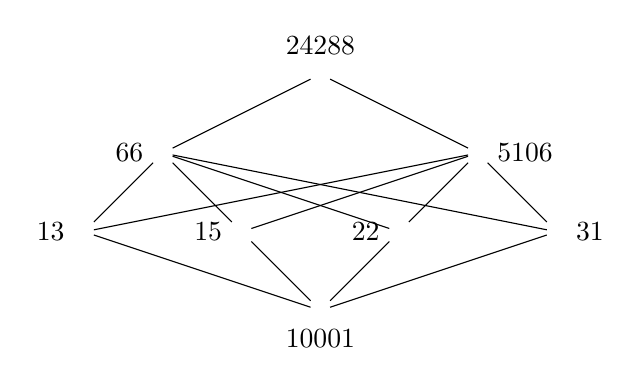
\begin{tikzpicture}
        % Nodi del livello più basso (10001)
        \node[label=below:{$10001$}](n10001) at (3,0) {}; % Posizionato al centro in basso

        % Nodi del livello intermedio (13, 15, 22, 31)
        \node[label=left:{$13$}](n13) at (0,1) {};
        \node[label=left:{$15$}](n15) at (2,1) {};
        \node[label=left:{$22$}](n22) at (4,1) {};
        \node[label=right:{$31$}](n31) at (6,1) {};

        % Nodi del livello superiore (66, 5106)
        \node[label=left:{$66$}](n66) at (1,2) {};
        \node[label=right:{$5106$}](n5106) at (5,2) {};

        % Nodi del livello più alto (24288)
        \node[label=above:{$24288$}](n24288) at (3,3) {};

        % Collegamenti da 10001 ai nodi del livello intermedio
        \draw (n10001)--(n13);
        \draw (n10001)--(n15);
        \draw (n10001)--(n22);
        \draw (n10001)--(n31);

        % Collegamenti da 13, 15, 22, 31 a 66
        \draw (n13)--(n66);
        \draw (n15)--(n66);
        \draw (n22)--(n66);
        \draw (n31)--(n66);

        % Collegamenti da 13, 15, 22, 31 a 5106
        \draw (n13)--(n5106);
        \draw (n15)--(n5106);
        \draw (n22)--(n5106);
        \draw (n31)--(n5106);

        % Collegamenti da 66 e 5106 a 24288
        \draw (n66)--(n24288);
        \draw (n5106)--(n24288);
    \end{tikzpicture}
\end{center}

Sì è un reticolo ed è complementato ma non distributivo.

\subsubsection*{Quinto punto}

\begin{center}
    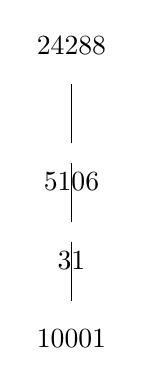
\begin{tikzpicture}
        % Nodi disposti verticalmente come nella figura
        \node[label=above:{$24288$}](n24288) at (0,3) {};
        \node[label=below:{$5106$}](n5106) at (0,2) {};
        \node[label=below:{$31$}](n31) at (0,1) {};
        \node[label=below:{$10001$}](n10001) at (0,0) {};

        % Collegamenti verticali
        \draw (n24288)--(n5106);
        \draw (n5106)--(n31);
        \draw (n31)--(n10001);
    \end{tikzpicture}
\end{center}

\subsubsection*{Sesto punto}

a = vuoto, vale tutto ciò che è stato detto al 4° punto.

\subsection*{Esercizio 5}

\subsubsection*{Punto 1}
L'elemento neutro rispetto alla somma è $\vec{0}_S = (0, 0, 0)$.
L'elemento neutro rispetto al prodotto è $\vec{1}_S = (0, 0, 1)$.

\subsubsection*{Punto 2}
Per l'elemento $(1, 2, -1)$, l'opposto è dato da $(a,b,c) + (a',b',c') = (0,0,0)$.
Per la prima componente: $1 + a' = 0 \implies a' = -1$.
Per la seconda componente: $2 + b' = 0 \implies b' = -2$.
Per la terza componente: $-1 + c' = 0 \implies c' = 1$.
Quindi, l'opposto di $(1, 2, -1)$ è $(-1, -2, 1)$.

L'inverso di $(1, 2, -1)$ deve soddisfare $(1, 2, -1) \cdot (a, b, c) = (0, 0, 1)$.
$(1 \cdot a, 1 \cdot b + 2 \cdot a, 1 \cdot c -1 \cdot a) = (a, b+2a, c-a) = (0, 0, 1)$.
$a=0$, $b+2a=0 \implies b=0$, $c-a=1 \implies c=1$.
L'inverso di $(1, 2, -1)$ è $(0, 0, 1)$.

\subsubsection*{Punto 3}
Per determinare se un elemento è un divisore dello zero, dobbiamo verificare se esiste un altro elemento non nullo che, moltiplicato per il primo, dà l'elemento neutro $(0,0,0)$.

Per $(1, 2, -1)$:
Supponiamo che esista un elemento $(a, b, c) \ne (0, 0, 0)$ tale che:
$(1, 2, -1) \cdot (a, b, c) = (a, b+2a, c-a) = (0, 0, 0)$.
Questo implica che:
$a = 0$
$b + 2a = 0 \implies b=0$
$c - a = 0 \implies c=0$
Quindi $(a, b, c) = (0, 0, 0)$. Non esiste un elemento non nullo che soddisfi la condizione, perciò $(1, 2, -1)$ **non** è un divisore dello zero.

Per $(1, 1, 0)$:
Supponiamo che esista un elemento $(a, b, c) \ne (0, 0, 0)$ tale che:
$(1, 1, 0) \cdot (a, b, c) = (a, b+a, c) = (0, 0, 0)$.
Questo implica che:
$a = 0$
$b + a = 0 \implies b=0$
$c = 0$
Quindi $(a, b, c) = (0, 0, 0)$. Anche in questo caso non esiste un elemento non nullo, quindi $(1, 1, 0)$ **non** è un divisore dello zero.

\section{Esame del 16 luglio 2025}
\begin{center}
	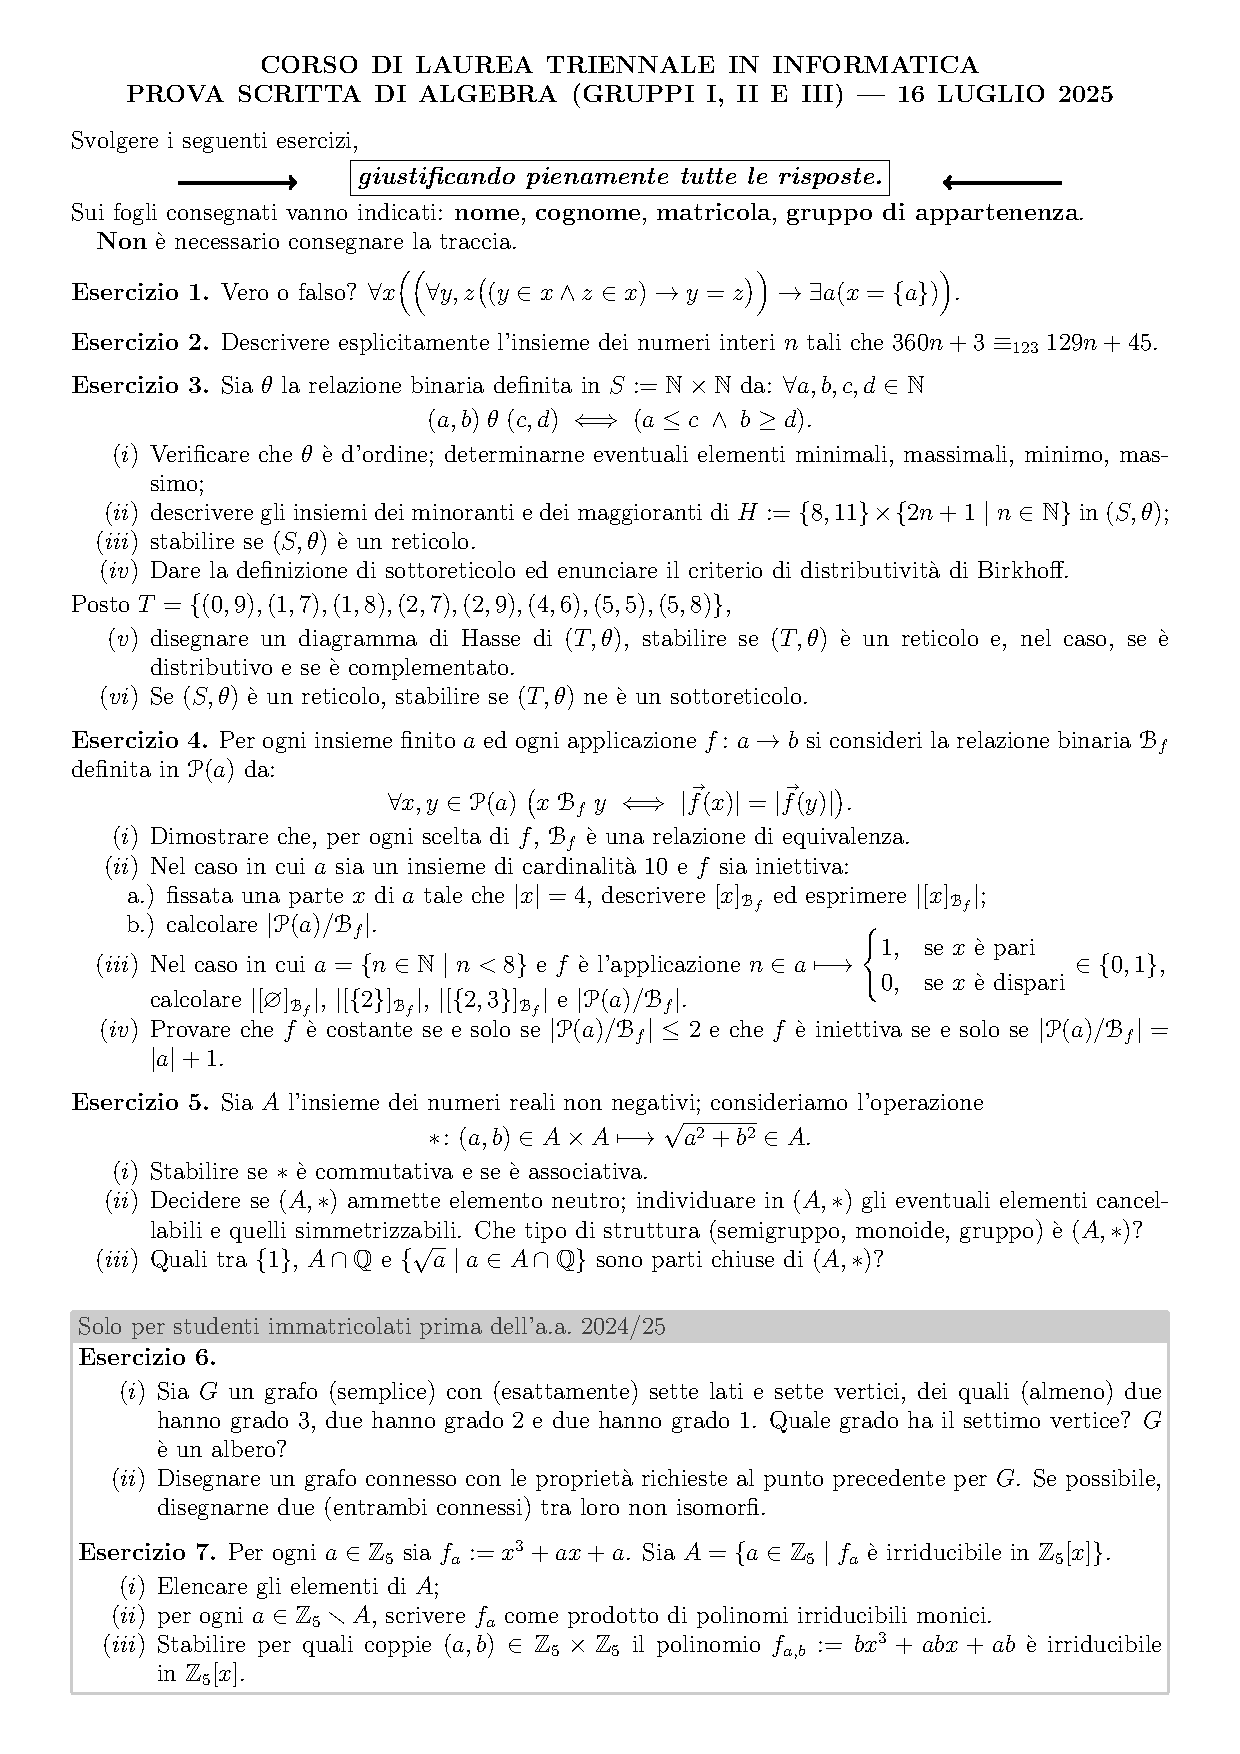
\includegraphics[scale=.85]{pdf/25-07-16.pdf}
\end{center}

\subsection*{Esercizio 1}
La proposizione $\forall x((\forall y,z((y\in x\wedge z\in x)\rightarrow y=z))\rightarrow\exists a(x=\{a\}))$ è falsa.
Per dimostrarlo, è sufficiente trovare un controesempio, cioè un insieme $x$ per cui la proposizione non è verificata.
Consideriamo l'insieme vuoto, $x = \emptyset$.
\begin{itemize}
    \item L'antecedente della prima implicazione, $(y\in x\wedge z\in x)$, è sempre falso perché non esistono elementi in $x$. Poiché l'antecedente è falso, l'implicazione $(y\in x\wedge z\in x)\rightarrow y=z$ è sempre vera.
    \item Di conseguenza, la proposizione quantificata $(\forall y,z((y\in x\wedge z\in x)\rightarrow y=z))$ è vera.
    \item Consideriamo ora il conseguente della seconda implicazione, $\exists a(x=\{a\})$. Se $x=\emptyset$, non esiste un elemento $a$ tale che $x=\{a\}$, quindi la proposizione è falsa.
\end{itemize}
La proposizione completa diventa quindi: $(\text{vero}) \rightarrow (\text{falso})$, che è falsa. Poiché non è vera per ogni $x$, la proposizione iniziale è falsa.

\subsection*{Esercizio 2}
Dobbiamo risolvere la congruenza $360n+3\equiv_{123}129n+45.$
\begin{itemize}
    \item Riscriviamo la congruenza: $360n - 129n \equiv 45 - 3 \pmod{123}$.
    \item Otteniamo: $231n \equiv 42 \pmod{123}$.
    \item Calcoliamo il Massimo Comun Divisore tra 231 e 123 utilizzando l'algoritmo di Euclide:
    \begin{itemize}
        \item $231 = 1 \cdot 123 + 108$
        \item $123 = 1 \cdot 108 + 15$
        \item $108 = 7 \cdot 15 + 3$
        \item $15 = 5 \cdot 3 + 0$
    \end{itemize}
    Il MCD è 3. Poiché $3$ divide 42, esistono soluzioni. Dividiamo per 3 tutti i termini della congruenza:
    \item $\frac{231}{3}n \equiv \frac{42}{3} \pmod{\frac{123}{3}}$
    \item $77n \equiv 14 \pmod{41}$.
    \item Per trovare $n$, dobbiamo calcolare l'inverso di $77 \pmod{41}$.
    $77 \equiv 36 \equiv -5 \pmod{41}$.
    Quindi, l'inverso di $-5 \pmod{41}$ è $8$, poiché $(-5) \cdot (-8) = 40 \equiv -1 \pmod{41}$. Oh, scusa, è $(-5) \cdot 8 = -40 \equiv 1 \pmod{41}$. Quindi l'inverso è $8$.
    \item Moltiplichiamo entrambi i membri della congruenza per 8:
    $8 \cdot 77n \equiv 8 \cdot 14 \pmod{41}$
    $1n \equiv 112 \pmod{41}$
    $112 = 2 \cdot 41 + 30$, quindi $112 \equiv 30 \pmod{41}$.
    \item Le soluzioni sono $n \equiv 30 \pmod{41}$.

\end{itemize}

\subsection*{Esercizio 3}
Sia la relazione binaria definita in $S:=\mathbb{N}\times\mathbb{N}$ da: $(a, b) \theta (c,d)\iff(a\le c\wedge b\ge d)$.
\begin{itemize}
    \item[(i)] \textbf{Verifica che è una relazione d'ordine:}
    \begin{itemize}
        \item \textbf{Riflessività:} $(a,b)\theta(a,b)$ è vero poiché $a\le a$ e $b\ge b$.
        \item \textbf{Antisimmetria:} Se $(a,b)\theta(c,d)$ e $(c,d)\theta(a,b)$, allora $a\le c$ e $b\ge d$, e $c\le a$ e $d\ge b$. Questo implica che $a=c$ e $b=d$, quindi $(a,b)=(c,d)$.
        \item \textbf{Transitività:} Se $(a,b)\theta(c,d)$ e $(c,d)\theta(e,f)$, allora $a\le c\le e$ e $b\ge d\ge f$. Questo implica che $a\le e$ e $b\ge f$, ovvero $(a,b)\theta(e,f)$.
    \end{itemize}
    La relazione è d'ordine. Non esistono elementi minimali, massimali, minimo o massimo, poiché per ogni $(a,b)$ esiste un elemento $(a-1, b+1)$ più piccolo e $(a+1, b-1)$ più grande, a meno che $a=0$.

    \item[(ii)] \textbf{Insiemi di minoranti e maggioranti di $H$:}
    Sia $H:=\{8,11\}\times\{2n+1|n\in\mathbb{N}\} = \{(8,1), (8,3), (8,5), \dots, (11,1), (11,3), (11,5), \dots\}$.
    \begin{itemize}
        \item \textbf{Minoranti:} L'insieme dei minoranti di $H$ è dato da $\{(a,b)\in S | (a,b)\theta(c,d) \forall (c,d)\in H\}$.
        Questo implica che $a\le c$ e $b\ge d$ per ogni $(c,d)\in H$. Per la prima componente, $a\le 8$ e $a\le 11$, quindi $a\le 8$. Per la seconda, $b\ge 2n+1$ per ogni $n\in\mathbb{N}$, il che è impossibile. L'insieme dei minoranti è l'insieme vuoto, $\emptyset$.
        \item \textbf{Maggioranti:} L'insieme dei maggioranti di $H$ è dato da $\{(a,b)\in S | (c,d)\theta(a,b) \forall (c,d)\in H\}$.
        Questo implica che $c\le a$ e $d\ge b$ per ogni $(c,d)\in H$. Questo è possibile per ogni coppie (a,b) t.c a >= 11 AND b <= 1
    \end{itemize}
    \item[(iii)] \textbf{È un reticolo?}
    No, $(S, \theta)$ non è un reticolo

	\item[(iv)] \textbf{Def sottoreticolo e Birkhoff} 
	La trovate nelle dispense

	\item[(v)] \textbf{Disegnare Hasse dell'insieme T:}
	
	\begin{center}
		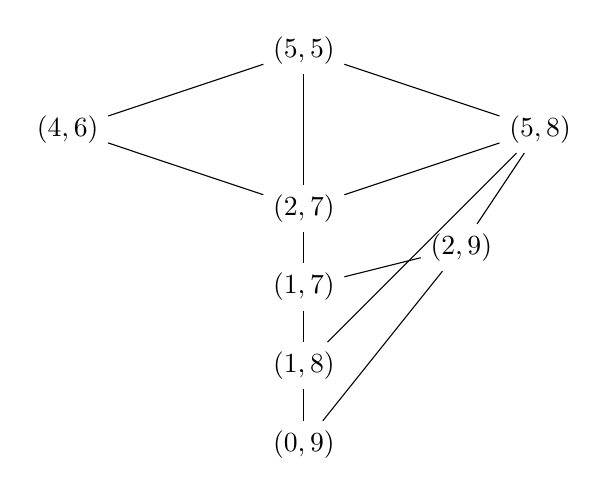
\begin{tikzpicture}
			% Nodi
			\node (n46) at (0,3) {$(4,6)$};
			\node (n55) at (3,4) {$(5,5)$};
			\node (n58) at (6,3) {$(5,8)$};
	
			\node (n27) at (3,2) {$(2,7)$};
			\node (n17) at (3,1) {$(1,7)$};
			\node (n18) at (3,0) {$(1,8)$};
			\node (n09) at (3,-1) {$(0,9)$};
			
			\node (n29) at (5,1.5) {$(2,9)$};
			
			% Collegamenti
			\draw (n46) -- (n27);
			\draw (n55) -- (n27);
			\draw (n58) -- (n27);
			
			\draw (n27) -- (n17);
			\draw (n17) -- (n18);
			\draw (n18) -- (n09);
			
			\draw (n58) -- (n29);
			\draw (n29) -- (n17);
			\draw (n18) -- (n58);
			\draw (n29) -- (n09);
			
			\draw (n46) -- (n55);
			\draw (n58) -- (n55);

		\end{tikzpicture}
	\end{center}

	Non è un reticolo perch avrà infiniti minimali visto che ad esempio (0, 0) e (0, 1) non sono in relazione

	\item[(vi)] \textbf{ Se (S, θ) è un reticolo, stabilire se (T, θ) ne è un sottoreticolo} 

	Non può essere un reticolo visto che quello "originale" non lo è e quindi non c'è alcun INF e SUP

\end{itemize}

\subsection*{Esercizio 4}
Per ogni insieme finito $a$ ed ogni applicazione $f:a\rightarrow b$ si consideri la relazione binaria $\mathcal{B}_{f}$ definita in $\mathcal{P}(a)$ da:
$\forall x,y\in\mathcal{P}(a)(x\mathcal{B}_{f}y\iff|f(x)|=|f(y)|)$.
\begin{itemize}
    \item[(i)] \textbf{Dimostrazione che $\mathcal{B}_{f}$ è una relazione di equivalenza:}
    \begin{itemize}
        \item \textbf{Riflessività:} Per ogni $x\in\mathcal{P}(a)$, $|f(x)|=|f(x)|$. Quindi $x\mathcal{B}_{f}x$.
        \item \textbf{Simmetria:} Per ogni $x,y\in\mathcal{P}(a)$, se $x\mathcal{B}_{f}y$, allora $|f(x)|=|f(y)|$. Questo implica $|f(y)|=|f(x)|$, quindi $y\mathcal{B}_{f}x$.
        \item \textbf{Transitività:} Per ogni $x,y,z\in\mathcal{P}(a)$, se $x\mathcal{B}_{f}y$ e $y\mathcal{B}_{f}z$, allora $|f(x)|=|f(y)|$ e $|f(y)|=|f(z)|$. Per la proprietà transitiva dell'uguaglianza, $|f(x)|=|f(z)|$, quindi $x\mathcal{B}_{f}z$.
    \end{itemize}
    Poiché le tre proprietà sono verificate, $\mathcal{B}_{f}$ è una relazione di equivalenza.

    \item[(ii)] \textbf{Nel caso in cui $a$ sia un insieme di cardinalità 10 e $f$ sia iniettiva:}
    \begin{itemize}
        \item a.) Sia $x$ una parte di $a$ tale che $|x|=4$. Poiché $f$ è iniettiva, $|f(x)|=|x|=4$.
        La classe di equivalenza $[x]_{\mathcal{B}_{f}}$ è l'insieme di tutte le parti $y\in\mathcal{P}(a)$ tali che $|f(y)|=|f(x)|=4$. Poiché $f$ è iniettiva, questo è equivalente a $|y|=4$.
        $[x]_{\mathcal{B}_{f}} = \{ y\in\mathcal{P}(a) \mid |y|=4 \}$.
        La cardinalità di questa classe è il numero di sottoinsiemi di $a$ con 4 elementi, che è dato dal coefficiente binomiale $\binom{10}{4}$:
        $|[x]_{\mathcal{B}_{f}}| = \binom{10}{4} = \frac{10!}{4!6!} = \frac{10\cdot9\cdot8\cdot7}{4\cdot3\cdot2\cdot1} = 210$.
        \item b.) Le classi di equivalenza sono determinate dalla cardinalità dell'immagine, che in questo caso è equivalente alla cardinalità dei sottoinsiemi di $a$. Poiché $|a|=10$, i sottoinsiemi possono avere cardinalità da 0 a 10. Pertanto, ci sono 11 classi di equivalenza, una per ogni possibile cardinalità, da 0 a 10.
        $|\mathcal{P}(a)/\mathcal{B}_{f}| = 11$.
    \end{itemize}

    \item[(iii)] \textbf{Nel caso in cui $a=\{n\in\mathbb{N}|n<8\}$ e $f$ è l'applicazione $n\mapsto\begin{cases}1,&se~n\text{ è pari}\\ 0,&se~n\text{ è dispari}\end{cases}$:}
    Sia $P=\{0,2,4,6\}$ e $D=\{1,3,5,7\}$. $|P|=4$ e $|D|=4$.
    \begin{itemize}
        \item \textbf{$|[\emptyset]_{\mathcal{B}_{f}}| $}: $f(\emptyset) = \emptyset$, quindi $|f(\emptyset)|=0$. La classe di equivalenza contiene tutti gli insiemi $y$ tali che $|f(y)|=0$. Questo accade solo se $y=\emptyset$. Quindi $|[\emptyset]_{\mathcal{B}_{f}}|=1$.
        \item \textbf{$|[\{2\}]_{\mathcal{B}_{f}}| $}: $f(\{2\}) = \{1\}$, quindi $|f(\{2\})|=1$. La classe contiene tutti i sottoinsiemi $y$ tali che $|f(y)|=1$. Questo accade se $y$ contiene solo elementi pari (escluso $\emptyset$) o solo elementi dispari (escluso $\emptyset$).
        I sottoinsiemi non vuoti di $P$ sono $2^4-1=15$.
        I sottoinsiemi non vuoti di $D$ sono $2^4-1=15$.
        $|[\{2\}]_{\mathcal{B}_{f}}| = 15+15=30$.
        \item \textbf{$|[\{2,3\}]_{\mathcal{B}_{f}}|$}: $f(\{2,3\}) = \{1,0\}$, quindi $|f(\{2,3\})|=2$. La classe contiene tutti i sottoinsiemi $y$ tali che $|f(y)|=2$. Questo accade se $y$ contiene almeno un elemento pari e almeno un elemento dispari.
        Il numero totale di sottoinsiemi di $a$ è $2^8=256$.
        I sottoinsiemi che contengono solo elementi pari (e non il vuoto) sono 15.
        I sottoinsiemi che contengono solo elementi dispari (e non il vuoto) sono 15.
        L'unico sottoinsieme che produce un'immagine vuota è l'insieme vuoto stesso.
        Il numero di insiemi con cardinalità $|f(y)|=2$ è $2^8 - (2^4-1) - (2^4-1) - 1 = 256 - 15 - 15 - 1 = 225$.
        $|[\{2,3\}]_{\mathcal{B}_{f}}|=225$.
        \item \textbf{$|\mathcal{P}(a)/\mathcal{B}_{f}|$}: Il numero di classi di equivalenza è il numero di possibili cardinalità delle immagini. Le immagini possono essere $\emptyset$, $\{0\}$, $\{1\}$, o $\{0,1\}$. Le loro cardinalità sono rispettivamente 0, 1, 1, 2. Quindi, le possibili cardinalità dell'immagine sono 0, 1, 2. Questo significa che ci sono 3 classi di equivalenza.
        $|\mathcal{P}(a)/\mathcal{B}_{f}|=3$.
    \end{itemize}
\end{itemize}

\subsection*{Esercizio 5}
Sia $A$ l'insieme dei numeri reali non negativi; consideriamo l'operazione $*:(a,b)\in A\times A\mapsto\sqrt{a^{2}+b^{2}}\in A$.
\begin{itemize}
    \item[(i)] \textbf{Commutativa e associativa:}
    \begin{itemize}
        \item \textbf{Commutativa:} $a*b = \sqrt{a^2+b^2} = \sqrt{b^2+a^2} = b*a$. L'operazione è commutativa.
        \item \textbf{Associativa:} $(a*b)*c = \sqrt{(a*b)^2+c^2} = \sqrt{(\sqrt{a^2+b^2})^2+c^2} = \sqrt{a^2+b^2+c^2}$.
        $a*(b*c) = \sqrt{a^2+(b*c)^2} = \sqrt{a^2+(\sqrt{b^2+c^2})^2} = \sqrt{a^2+b^2+c^2}$.
        L'operazione è associativa.
    \end{itemize}
    \item[(ii)] \textbf{Struttura algebrica:}
    \begin{itemize}
        \item \textbf{Elemento neutro:} L'elemento neutro $e$ è tale che $a*e = a$ per ogni $a\in A$.
        $\sqrt{a^2+e^2}=a \implies a^2+e^2=a^2 \implies e^2=0 \implies e=0$. L'elemento neutro è $0$.
        \item \textbf{Elementi simmetrizzabili:} Un elemento $a$ è simmetrizzabile se esiste $a'$ tale che $a*a'=0$.
        $\sqrt{a^2+a'^2}=0 \implies a^2+a'^2=0$. Dato che $a,a' \ge 0$, l'unica soluzione è $a=0$ e $a'=0$.
        Solo l'elemento $0$ è simmetrizzabile.
    \end{itemize}
    Poiché l'operazione è associativa, ha un elemento neutro ed è commutativa, la struttura $(A, *)$ è un **monoide abeliano**.

    \item[(iii)] \textbf{Parti chiuse:}
    \begin{itemize}
        \item \textbf{$\{1\}$:} Non è chiusa. $1*1 = \sqrt{1^2+1^2} = \sqrt{2}$, che non appartiene a $\{1\}$.
        \item \textbf{$A\cap\mathbb{Q}$:} Non è chiusa. Ad esempio, $1\in A\cap\mathbb{Q}$, ma $1*1=\sqrt{2}$, che non è un numero razionale.
        \item \textbf{$\{\sqrt{a}|a\in A\cap\mathbb{Q}\}$:} È chiusa. Siano $x,y$ due elementi dell'insieme. Allora $x=\sqrt{a}$ e $y=\sqrt{b}$ con $a,b\in\mathbb{Q}$ e $a,b\ge 0$.
        $x*y=\sqrt{x^2+y^2}=\sqrt{(\sqrt{a})^2+(\sqrt{b})^2}=\sqrt{a+b}$.
        Dato che la somma di due numeri razionali è un numero razionale, $a+b$ è un numero razionale non negativo. Quindi $\sqrt{a+b}$ appartiene all'insieme. L'insieme è chiuso.
    \end{itemize}
\end{itemize}
